\chapter{Analysis}
\label{chap:analysis}

\section{Methodology}

\subsection{Performance gained by using multiple levels of detail}
\label{sec:analysis-mipmap}
The perception module (section~\ref{sec:arch-perception}) of this work detects objects by matching their photos against camera images using the SIFT method (section~\ref{sec:impl-sift}). Matching images against each other is a very performance intensive task. Let $I_1$ and $I_2$ be two images, $K_1$ and $K_2$ the corresponding sets of keypoints and $m_1 = |K_1|$ and $m_2 = |K_2|$ the maximum number of keypoints in each set. The maximum number of keypoints per set is limited by the size of the image: $m_1 <= |I_1|$ and $m_2 <= |I_2|$. Sample images are never larger than the camera images they are matched against (section~\ref{sec:impl-db-limits}), therefore it is established that one image is at most as large as the other: $|I_1| <= |I_2|$. In conclusion, the complexity for the worst case is $O(m^2)$ with $m = m_1 = m_2$.

In order to be able to match multiple images in a sufficiently fast manner, $m$ is reduced by initially scaling down the images. The full sized images are only used if an object is detect in the scaled down version, to improve the projection from sample to camera image (section~\ref{sec:impl-mipmap}). This technique highly increases performance for larger databases of sample images. \\

To review the actual benefit of this method, the performance of the system needs to be quantified. The speed of execution of a computer program can be expressed in frames per second (FPS), a standard measurement for performance in real-time applications. It denotes the number of images processed in one second, where, in this case, ``images'' means camera images and ``processed'' matched against the entire set of sample images.

The increase in speed becomes visible when average FPS are measured for both configurations - with downscaling and without - and plotted against each other. Comparable results can be obtained by defining standard situations to be used in both configurations. The performance of the system depends on two parameters: The amount of sample images in the database and the number of currently visible objects. Situations of interest are any combination of large, medium and small databases and no, one and multiple visible objects. In order not to distort the results, the same objects should be used in both configurations, as well as the same distance to the visible objects. \\

It can be expected, that the performance without visible objects is much higher with downscaling, because then this method definitely needs to match less keypoints. On the other hand, when using downscaling and objects are visible, they will trigger the use of larger images, causing the performance to drop. For smaller databases, the speed might drop even below the speed without downscaling: If, for example, only one object exists in the database and this object is visible, then the configuration with downscaling will need to match both sizes, the configuration without downscaling only the original size.


\subsection{Stability improvements through ``tracking'' findings from previous frames}
\label{sec:analysis-tracking}
Section~\ref{sec:impl-mipmap} details how the system tries to detect objects that were successfully recognized in the previous frame. This method is supposed to stabilize the perception, i.e. increase the chance to detect currently visible objects. \\

To measure the success of this rudimentary tracking method, a situation can be created where it is known which objects are currently visible. An ideal output of the system can be derived from the definition of this situation. Then, when running the system with and without tracking, its output can be compared with the ideal output to calculate how close both variants come. Dropped frames, i.e. frames where a visible object was not successfully recognized, can be visualized with a binary graph (the x-axis indicating frames and the y-axis indicating if a specific object was detected). A consistent graph would indicate a stable perception, a ``busy'' graph would indicate a lot of dropped frames. \\

Distant objects are more difficult to detect, because they appear smaller on the camera image and exhibit less distinctive features to be matched against a sample. Therefore it can be expected, that the amount of dropped frames increases with a higher distance to the object. In order to get comparable results, distance and angle between camera and object need to be the same for tests with and without tracking. Situations with both, close and far distances, need to be tested: The improvement in stability with tracking should get higher for far distances (the perception of close objects is pretty stable even without tracking).


\subsection{Decrease in false-positives through discarding concave projections}
Sometimes the SIFT method (section~\ref{sec:impl-sift}) finds false matches that cause the detection of objects that are not currently visible. Because this work deals with rectangular objects only, many errors can be identified by projecting recognized objects onto the camera image and checking if its corners form a convex quadrangle and no two opposite sites intersect (see section~\ref{sec:impl-2Dpose}). \\

Evaluating the ratio of discarded false positives works analogues to the evaluation of the tracking method (see section~\ref{sec:analysis-tracking}): A situation is created where it is known which objects are currently visible. However, \underline{not} visible objects are compared with detected objects, in order to identify false positives. The resulting graph is perfectly flat if all false positives are discarded.


\subsection{Better 3D pose approximations by queueing multiple findings}
SIFT matches can contain a lot of noise and OpenNI laser sensors are not very accurate. Both are causes for distortion when calculating the 3D pose of an object. Therefore, the semantic map keeps multiple poses of one object, enabling it to calculate an average and cancel out the noise (as detailed in section~\ref{sec:impl-queue}). \\

By placing a new object in front of the camera during runtime, the change of the 3D pose assigned to this object by the semantic map can be observed. The pose should change rapidly at first, then approach a stable state. To illustrate this behaviour, the output of the system can be turned into a graph, where the x-axis represents time and the y-axis one parameter of the pose (thus, the result would consist of 3 graphs displaying the position and 3 graphs displaying the direction vector).

If the position of an object is established, the pose calculated by the system can be compared to the real pose. Thereby the quality of the approximation of a pose can be evaluated as well. \\

It is expected, that the observed pose approaches a stable state for a static scene, but might change when introducing camera movement. The system can only estimate a pose, because the result of its calculations depend on the quality of the SIFT matches (see section~\ref{sec:impl-sift}) and the depth image (the laser sensor produces better results for front-facing surfaces as opposed to surfaces rotated away from the camera). \\


%\subsection{Less false-positives by removing unconfirmed objects}
%Although many false positives can be discarded early, some get through the filters, get published by the perception and end up in the semantic map. Others are correctly recognized but change their position afterwards. The semantic map tries to identify these cases by checking if objects are detected more than once. Otherwise they get removed again (described in section~\ref{sec:impl-memo}). \\


\subsection{Relevance of objects suggested by the evaluation function}
Users who need a specific object can query the semantic map to find out it can remember seeing such an object before. If multiple objects of this type were seen before, the semantic map suggests where to look first, by evaluating all candidates based on spatial and temporal distance (section~\ref{sec:impl-eval}). \\

To assess if the evaluation function employed by the semantic map suggests the best candidates, a scene with a representative range of objects of one type can created. Representative means that objects for all possible extreme cases should be included in this scene, i.e. any combination of close / far locations and short / long times since these objects where detected. Because dealing with long distances and time spans is difficult in the lab, the necessary objects can be inserted artificially into the system. \\

It is expected, that the evaluation function will primarily favour close objects, but prefer more recently seen objects to previously seen objects, because it weighs spatial distance higher than temporal distance.


\section{Experimentation}

\begin{figure}[H]
  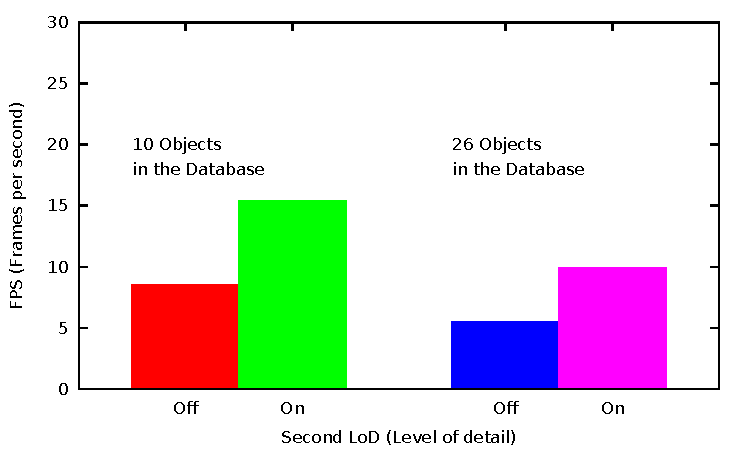
\includegraphics[width=1.0\textwidth]{images/fps-0-objects.pdf}
  \caption{FPS with 0 visible objects}
\end{figure}

\begin{figure}[H]
  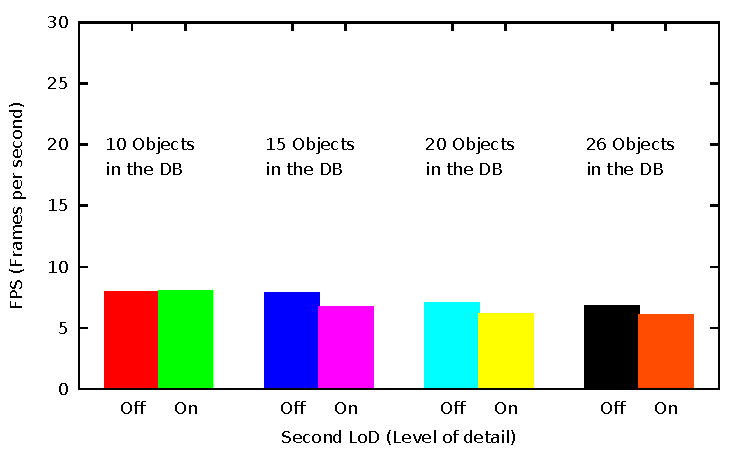
\includegraphics[width=1.0\textwidth]{images/fps-2-objects.pdf}
  \caption{FPS with 2 visible objects}
\end{figure}

\begin{figure}[H]
  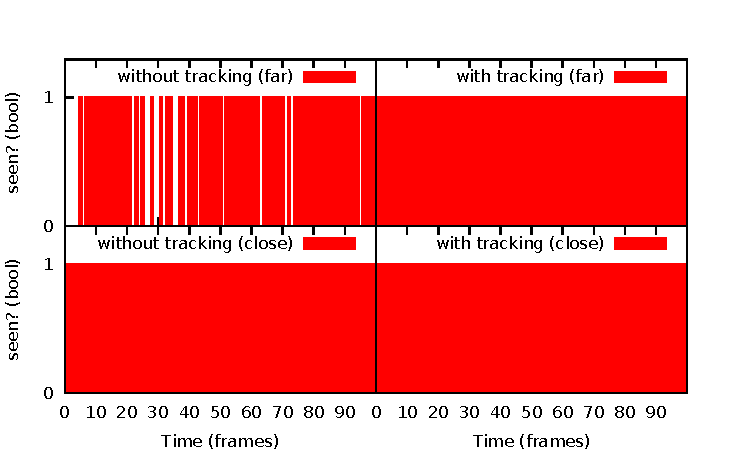
\includegraphics[width=1.0\textwidth]{images/perceptions.pdf}
  \caption{Successful objects detections with and without ``tracking''}
\end{figure}

\begin{figure}[H]
  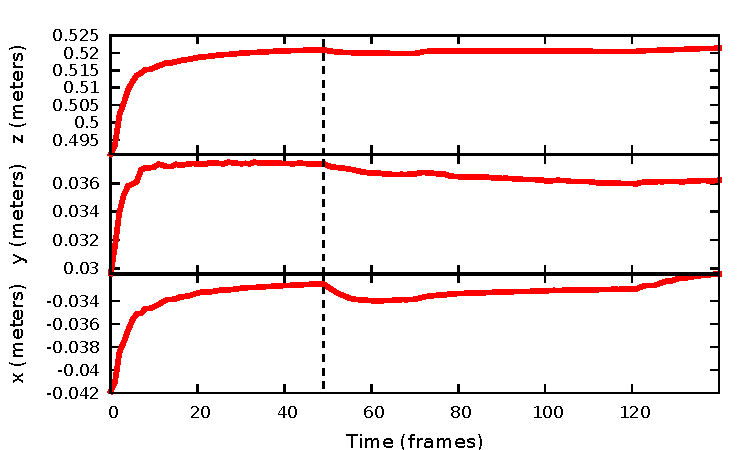
\includegraphics[width=1.0\textwidth]{images/3D-poses-position.pdf}
  \caption[3D poses position convergence]{3D pose position approximation. At around 50 frames, the position of the object changed slightly. Up until and after that point, the values converged to the real position.}
\end{figure}

\begin{figure}[H]
  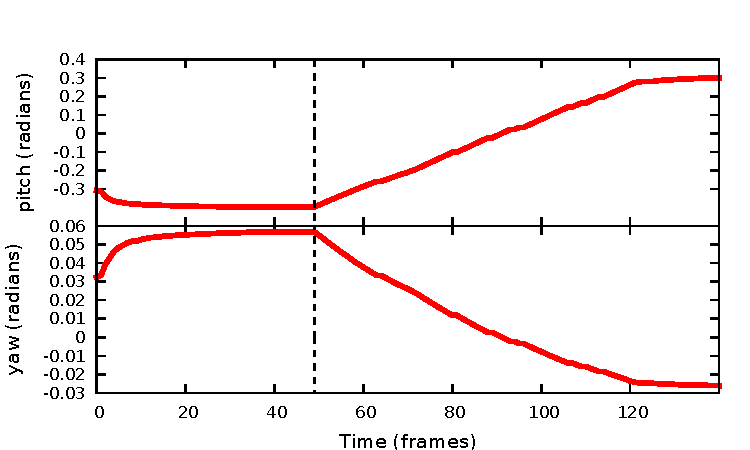
\includegraphics[width=1.0\textwidth]{images/3D-poses-orientation.pdf}
  \caption[3D poses orientation convergence]{3D pose orientation approximation. At around 50 frames, the orientation of the object changed. Up until and after that point, the values converged to the real orientation.}
\end{figure}
%\subsection{PR2}
%\subsection{RGB-D SLAM}

\section{Evaluation}


